\documentclass[conference]{IEEEtran}

\usepackage{graphicx}
\usepackage{booktabs}
\usepackage{amsmath}
\usepackage{url}
\usepackage{xcolor}

\graphicspath{{../results/figures/}}
\newcommand{\todo}[1]{\textcolor{red}{[TODO: #1]}}

% Team draft merged into the template. Comments marked FACTS are notes for fixing the text;
% they do not appear in the PDF. Compile on Overleaf with paper/ and results/ uploaded
% (keep the folder layout), main file paper/main.tex.

\begin{document}

\title{CodeMigrate: Evidence-Grounded Detection of Breaking API Changes in Django Upgrades}

\author{
\IEEEauthorblockN{Author Name}
\IEEEauthorblockA{
Department of Computer Science and Engineering\\
University Name\\
India\\
author@example.com
}
}

\maketitle

\begin{abstract}

% FACTS: results exist -- F1 0.82 vs 0.02 (django-upgrade); hallucinated findings
% 29% (LLM only) -> 6% (RAG) -> 0% (RAG + validator). Replace "is designed" / "aims to".

Framework upgrades frequently introduce breaking API changes
that affect existing software applications. Although official
release notes document these changes, developers often lack
automated tools capable of detecting them reliably.

This paper presents CodeMigrate, an evidence-grounded
framework for identifying breaking API changes during
Django upgrades.

CodeMigrate combines Abstract Syntax Tree (AST) analysis,
retrieval from a structured knowledge base, and
Large Language Model (LLM) reasoning.

The knowledge base contains 310 sourced Django API changes
covering versions 4.0 through 5.2.

The proposed system uses deterministic citation validation
to ensure that generated findings are supported by
retrieved documentation.

Evaluation is designed around a benchmark of 235 cases
labeled through execution under different Django versions.

The framework aims to improve migration detection accuracy
while reducing unsupported claims generated by LLMs.

\end{abstract}

\begin{IEEEkeywords}
Django, API Migration, Large Language Models,
Retrieval-Augmented Generation, Static Analysis,
Software Maintenance
\end{IEEEkeywords}

\section{Introduction}

Software frameworks evolve continuously to introduce
new features, improve performance, and address security
vulnerabilities.

However, framework upgrades may introduce breaking API
changes that cause previously working applications to fail.

Django follows a structured release cycle in which
deprecated APIs are eventually removed.

Developers must identify incompatible API usage before
upgrading applications.

Existing automated migration tools typically support
a predefined collection of transformations~\cite{djangoupgrade,pyupgrade}.

Large Language Models provide more flexible reasoning
capabilities but may generate unsupported migration
recommendations~\cite{wang2025deprecated,spracklen2025package}.

To address these limitations, we propose CodeMigrate,
an evidence-grounded framework for detecting breaking
API changes.

The primary contributions of this work are:

\begin{enumerate}

\item A structured knowledge base containing 310
documented Django API changes.

\item An AST-based code analysis pipeline for detecting
potentially incompatible API usage.

\item An evidence-grounded LLM reasoning mechanism.

\item A deterministic citation validation framework.

\item A benchmark consisting of 235 migration cases.

\end{enumerate}

\section{Background and Related Work}

% FACTS (docs/RELATED_WORK.md): add LLM-and-API-change work and say how we differ --
% \cite{wang2025deprecated} deprecated APIs in LLM completion; \cite{liu2024codeupdatearena}
% update docs in prompt don't help; \cite{islah2024gitchameleon} version-specific generation
% (GPT-4o pass@10 39.9%); \cite{spracklen2025package} package hallucination (21.7% open-source);
% \cite{chen2025apidocs} RAG over API docs (+83--220%); \cite{islam2025migratelib} library
% migration (32% fully correct). Gap: none checks each LLM claim against the cited evidence
% and the code line, and none labels a framework upgrade by execution.

\subsection{API Evolution}

Application Programming Interfaces evolve as software
frameworks introduce new capabilities and remove
outdated functionality~\cite{dig2006apis}.

API changes can introduce compatibility problems
when applications depend on removed or modified methods.

\subsection{Automated Code Migration}

Automated migration tools analyze source code and
apply predefined transformations.

Examples include django-upgrade~\cite{djangoupgrade} and pyupgrade~\cite{pyupgrade}.

However, rule-based approaches may not cover every
documented API change.

\subsection{Retrieval-Augmented Generation}

Retrieval-Augmented Generation combines external
knowledge retrieval with language model reasoning~\cite{lewis2020rag}.

This approach allows generated responses to be
grounded in relevant documentation.

\section{Proposed Approach}

CodeMigrate consists of five major components.

\subsection{Knowledge Base Construction}

The knowledge base is constructed using official
Django release documentation.

Each entry contains information about an API change,
including its affected version, change type,
severity, and possible migration strategy.

% FACTS: 293 auto-parsed / 13 corrected / 4 manual; Table~\ref{tab:kb}.
% Numbers from `codemigrate kb stats` (KB built from Django commit 79502d0).
\begin{table}[t]
\centering
\small
\caption{Knowledge-base entries by Django release and change type.}
\label{tab:kb}
\begin{tabular}{lrrrrr}
\toprule
Version & Behavior & Deprecated & Removed & Renamed & Total \
\midrule
4.0 & 28 & 24 & 25 & 3 & 80 \
4.1 & 27 & 16 & 5 & 2 & 50 \
4.2 & 5 & 19 & 5 & 0 & 29 \
5.0 & 28 & 14 & 34 & 3 & 79 \
5.1 & 12 & 13 & 20 & 0 & 45 \
5.2 & 21 & 6 & 0 & 0 & 27 \
\midrule
Total & 121 & 92 & 89 & 8 & 310 \
\bottomrule
\end{tabular}
\end{table}


\subsection{Static Code Analysis}

CodeMigrate uses Abstract Syntax Tree analysis
to identify API references in Python source code.

The analyzer examines imports, function calls,
attribute access, and class definitions.

\subsection{Evidence Retrieval}

Relevant API changes are retrieved using a
combination of exact symbol matching,
BM25 ranking~\cite{robertson2009bm25}, and dense vector
retrieval~\cite{reimers2019sbert,johnson2019faiss}.

Reciprocal Rank Fusion~\cite{cormack2009rrf} combines results from
multiple retrieval methods.

\subsection{LLM-Based Reasoning}

Retrieved evidence and source code context are
provided to a Large Language Model.

The model identifies potential compatibility issues
and produces structured findings.

\subsection{Citation Validation}

% FACTS: a finding is VERIFIED only if the cited entry (1) was retrieved for that code line,
% (2) names the API used on that line, (3) is inside the version range; otherwise UNVERIFIED
% (bad citation) or UNSUPPORTED_CLAIM (no citation) and dropped.

A deterministic validation component checks whether
each generated finding is supported by retrieved
evidence.

Findings are classified according to their
verification status.

\section{Benchmark}

% FACTS: runs under Django 4.0.10, 4.1.13, 4.2.30, 5.0.14, 5.1.15; 168 positive lines;
% dev 75 / test 160 cases; Table~\ref{tab:dataset}.

The evaluation benchmark contains 235 migration cases.

Cases are labeled using execution results from
different Django versions.

The benchmark includes examples of deprecated APIs,
removed functionality, and compatible code.

The dataset is divided into development and
testing subsets.

% Numbers from benchmark/README.md (python -m benchmark.dataset_card).
\begin{table}[t]
\centering
\small
\caption{Benchmark cases used in the evaluation (status \texttt{ok}).}
\label{tab:dataset}
\begin{tabular}{llrr}
\toprule
Split & Kind & Cases & Positive labels \
\midrule
dev & real & 31 & 12 \
dev & synthetic & 35 & 60 \
dev & negative & 9 & 0 \
test & real & 67 & 3 \
test & synthetic & 70 & 93 \
test & negative & 23 & 0 \
\midrule
\multicolumn{2}{l}{Total} & 235 & 168 \
\bottomrule
\end{tabular}
\end{table}


\section{Experimental Evaluation}

\subsection{Research Questions}

The evaluation investigates four research questions.

\begin{enumerate}

\item How accurately does CodeMigrate detect
breaking API changes?

\item Does citation validation reduce unsupported
LLM-generated findings?

\item Which retrieval configuration provides
the best detection performance?

\item What are the computational costs and
latency of the proposed approach?

\end{enumerate}

\subsection{Baseline Systems}

% FACTS: A = django-upgrade, pyupgrade; B = LLM only; C = RAG, no validator; D = full
% pipeline; LLM = gemini-3.5-flash-lite, temperature 0, one run.

CodeMigrate is compared against automated migration
tools and LLM-based approaches.

The evaluation includes:

\begin{itemize}

\item Rule-based migration tools.

\item An LLM without retrieval.

\item Retrieval-Augmented Generation without validation.

\item The complete CodeMigrate pipeline.

\end{itemize}

\subsection{Evaluation Metrics}

Detection performance is measured using precision,
recall, and F1-score.

Precision is calculated as:

\begin{equation}
P = \frac{TP}{TP + FP}
\end{equation}

Recall is calculated as:

\begin{equation}
R = \frac{TP}{TP + FN}
\end{equation}

The F1-score is calculated as:

\begin{equation}
F_1 = \frac{2PR}{P + R}
\end{equation}

Additional metrics include hallucination rate,
citation accuracy, execution latency, and cost.

\begin{table}[t]
\centering
\small
\caption{System comparison on the test split (execution-labeled).}
\label{tab:comparison-test}
\begin{tabular}{lrrrrrrrr}
\toprule
System & Runs & P (\%) & R (\%) & F1 (\%) & F1 95\% CI & Halluc. (\%) & Cit. acc. (\%) & Exact line (\%) \\
\midrule
A-django-upgrade & 1 & 9.1 & 1.0 & 1.9 & [0.0, 6.1] & n/a & n/a & 100.0 \\
A-pyupgrade & 1 & 0.0 & 0.0 & 0.0 & [0.0, 0.0] & n/a & n/a & 0.0 \\
D-full[offline] & 1 & 75.2 & 88.5 & 81.3 & [74.0, 88.1] & 0.0 & 100.0 & 98.8 \\
C-rag-no-validator[offline] & 1 & 75.2 & 88.5 & 81.3 & [74.0, 88.1] & 0.0 & n/a & 98.8 \\
B-llm-only[gemini] & 1 & 68.3 & 74.0 & 71.0 & [63.1, 77.6] & 29.4 & n/a & 100.0 \\
C-rag-no-validator[gemini] & 1 & 76.5 & 91.7 & 83.4 & [77.1, 89.0] & 5.6 & 94.4 & 98.9 \\
D-full[gemini] & 1 & 77.8 & 87.5 & 82.4 & [75.4, 88.2] & 0.0 & 100.0 & 98.8 \\
\bottomrule
\end{tabular}
\end{table}

\begin{table}[t]
\centering
\small
\caption{Ablations (test split).}
\label{tab:ablations-test}
\begin{tabular}{lrrrrrrrr}
\toprule
system & ablation & retriever & top\_k & precision & recall & f1 & halluc & findings \\
\midrule
D[offline] & retriever & exact & 5 & 70.8 & 88.5 & 78.7 & 0.0 & 158 \\
D[offline] & retriever & bm25 & 5 & 70.8 & 88.5 & 78.7 & 0.0 & 158 \\
D[offline] & retriever & tfidf & 5 & 70.8 & 88.5 & 78.7 & 0.0 & 158 \\
D[offline] & retriever & dense & 5 & 73.3 & 88.5 & 80.2 & 0.0 & 153 \\
D[offline] & retriever & hybrid\_tfidf & 5 & 70.8 & 88.5 & 78.7 & 0.0 & 158 \\
D[offline] & retriever & hybrid & 5 & 70.8 & 88.5 & 78.7 & 0.0 & 158 \\
D[offline] & top\_k & hybrid & 1 & 70.8 & 88.5 & 78.7 & 0.0 & 158 \\
D[offline] & top\_k & hybrid & 3 & 70.8 & 88.5 & 78.7 & 0.0 & 158 \\
D[offline] & top\_k & hybrid & 5 & 70.8 & 88.5 & 78.7 & 0.0 & 158 \\
\bottomrule
\end{tabular}
\end{table}

\begin{table}[t]
\centering
\small
\caption{Recall by label evidence type and first failing version (test).}
\label{tab:breakdown-test}
\begin{tabular}{lrrrr}
\toprule
system & dimension & value & labels & recall \\
\midrule
A-django-upgrade & evidence & error & 74 & 1.4 \\
A-django-upgrade & evidence & warning only & 22 & 0.0 \\
A-django-upgrade & first version & 4.0.10 & 14 & 0.0 \\
A-django-upgrade & first version & 4.1.13 & 21 & 4.8 \\
A-django-upgrade & first version & 4.2.30 & 15 & 0.0 \\
A-django-upgrade & first version & 5.0.14 & 22 & 0.0 \\
A-django-upgrade & first version & 5.1.15 & 24 & 0.0 \\
A-pyupgrade & evidence & error & 74 & 0.0 \\
A-pyupgrade & evidence & warning only & 22 & 0.0 \\
A-pyupgrade & first version & 4.0.10 & 14 & 0.0 \\
A-pyupgrade & first version & 4.1.13 & 21 & 0.0 \\
A-pyupgrade & first version & 4.2.30 & 15 & 0.0 \\
A-pyupgrade & first version & 5.0.14 & 22 & 0.0 \\
A-pyupgrade & first version & 5.1.15 & 24 & 0.0 \\
D-full[offline] & evidence & error & 74 & 90.5 \\
D-full[offline] & evidence & warning only & 22 & 81.8 \\
D-full[offline] & first version & 4.0.10 & 14 & 71.4 \\
D-full[offline] & first version & 4.1.13 & 21 & 76.2 \\
D-full[offline] & first version & 4.2.30 & 15 & 93.3 \\
D-full[offline] & first version & 5.0.14 & 22 & 100.0 \\
D-full[offline] & first version & 5.1.15 & 24 & 95.8 \\
C-rag-no-validator[offline] & evidence & error & 74 & 90.5 \\
C-rag-no-validator[offline] & evidence & warning only & 22 & 81.8 \\
C-rag-no-validator[offline] & first version & 4.0.10 & 14 & 71.4 \\
C-rag-no-validator[offline] & first version & 4.1.13 & 21 & 76.2 \\
C-rag-no-validator[offline] & first version & 4.2.30 & 15 & 93.3 \\
C-rag-no-validator[offline] & first version & 5.0.14 & 22 & 100.0 \\
C-rag-no-validator[offline] & first version & 5.1.15 & 24 & 95.8 \\
B-llm-only[gemini] & evidence & error & 74 & 82.4 \\
B-llm-only[gemini] & evidence & warning only & 22 & 45.5 \\
B-llm-only[gemini] & first version & 4.0.10 & 14 & 100.0 \\
B-llm-only[gemini] & first version & 4.1.13 & 21 & 52.4 \\
B-llm-only[gemini] & first version & 4.2.30 & 15 & 73.3 \\
B-llm-only[gemini] & first version & 5.0.14 & 22 & 77.3 \\
B-llm-only[gemini] & first version & 5.1.15 & 24 & 75.0 \\
C-rag-no-validator[gemini] & evidence & error & 74 & 91.9 \\
C-rag-no-validator[gemini] & evidence & warning only & 22 & 90.9 \\
C-rag-no-validator[gemini] & first version & 4.0.10 & 14 & 92.9 \\
C-rag-no-validator[gemini] & first version & 4.1.13 & 21 & 85.7 \\
C-rag-no-validator[gemini] & first version & 4.2.30 & 15 & 100.0 \\
C-rag-no-validator[gemini] & first version & 5.0.14 & 22 & 95.5 \\
C-rag-no-validator[gemini] & first version & 5.1.15 & 24 & 87.5 \\
D-full[gemini] & evidence & error & 74 & 87.8 \\
D-full[gemini] & evidence & warning only & 22 & 86.4 \\
D-full[gemini] & first version & 4.0.10 & 14 & 78.6 \\
D-full[gemini] & first version & 4.1.13 & 21 & 85.7 \\
D-full[gemini] & first version & 4.2.30 & 15 & 93.3 \\
D-full[gemini] & first version & 5.0.14 & 22 & 95.5 \\
D-full[gemini] & first version & 5.1.15 & 24 & 83.3 \\
\bottomrule
\end{tabular}
\end{table}

\begin{table}[t]
\centering
\small
\caption{Latency, tokens and cost per case (test split).}
\label{tab:cost-test}
\begin{tabular}{lrrrrr}
\toprule
System & Latency/case (s) & Tokens/case & Cost/case (USD) & Findings & Rejected claims \\
\midrule
A-django-upgrade & 0.2 & 0.0 & 0.00000 & 37.0 & 0.0 \\
A-pyupgrade & 0.2 & 0.0 & 0.00000 & 129.0 & 0.0 \\
D-full[offline] & 0.1 & 0.0 & 0.00000 & 150.0 & 0.0 \\
C-rag-no-validator[offline] & 0.0 & 0.0 & 0.00000 & 150.0 & 0.0 \\
B-llm-only[gemini] & 0.0 & 1323.0 & 0.00000 & 119.0 & 0.0 \\
C-rag-no-validator[gemini] & 0.0 & 10704.0 & 0.00000 & 143.0 & 0.0 \\
D-full[gemini] & 0.0 & 10704.0 & 0.00000 & 135.0 & 8.0 \\
\bottomrule
\end{tabular}
\end{table}


\begin{figure}[t]
\centering
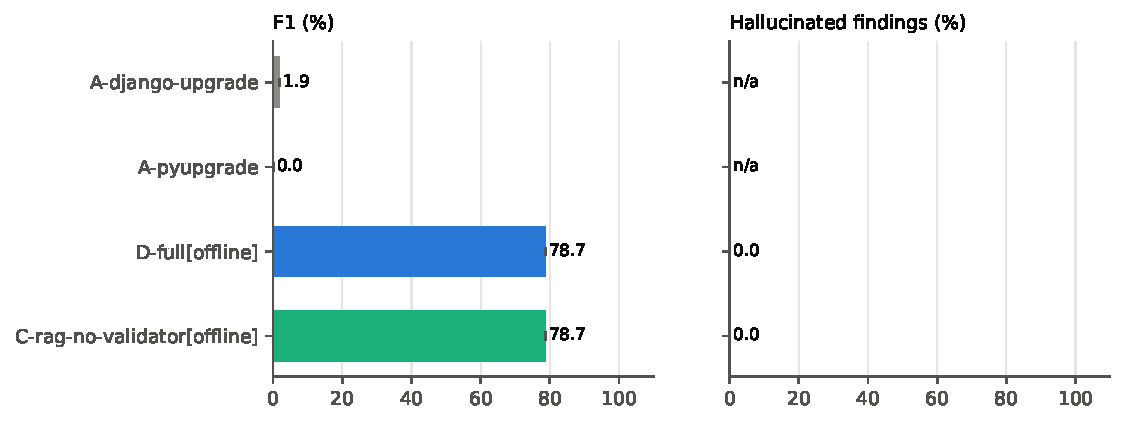
\includegraphics[width=\columnwidth]{f1_hallucination_test.pdf}
\caption{F1 vs.\ hallucination rate per system (test split).}
\label{fig:f1-halluc}
\end{figure}

\begin{figure}[t]
\centering
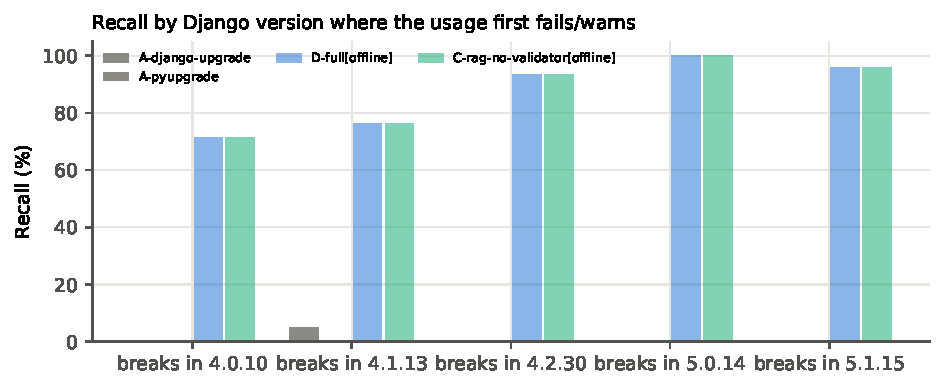
\includegraphics[width=\columnwidth]{breakdown_version_test.pdf}
\caption{Recall by the first Django version in which the usage breaks.}
\label{fig:by-version}
\end{figure}

\begin{figure}[t]
\centering
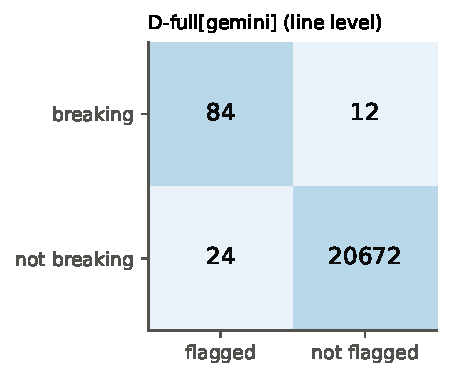
\includegraphics[width=0.8\columnwidth]{confusion_D-full_gemini_test.pdf}
\caption{Line-level confusion matrix of the full pipeline with Gemini (test split).}
\label{fig:confusion}
\end{figure}

\subsection{Results}

% FACTS (Table~\ref{tab:comparison-test}, test split, 160 cases):
% RQ1: D[gemini] F1 0.82 [0.75, 0.88] (P 0.78, R 0.88); D[offline] 0.81; django-upgrade 0.02,
%      pyupgrade 0.00; B 0.71.
% RQ2: hallucinated findings B 29.4% -> C 5.6% -> D 0.0%; validator rejected 8 claims; recall
%      0.92 -> 0.88; F1 difference not significant (paired bootstrap p = 0.82, McNemar p = 1.0).
% RQ3 (Table~\ref{tab:ablations-test}): dense F1 0.83, others 0.81; top-k 1/3/5 equal.
% RQ4 (Table~\ref{tab:cost-test}): offline 0.1 s/case; tokens/case 1,323 (B) vs 10,704 (C/D);
%      $0 on the free tier; Gemini latency 0.0 because replayed from cache.

\todo{Insert experimental results after evaluation.}

\section{Error Analysis}

% FACTS (results/error_cases.md, D[gemini]): 36 failures = 12 missed + 24 false positives;
% main cause: documented change that does not fail at runtime on that path (cached_property
% name argument, django-polymorphic); also dynamic access and KB gaps.

Potential sources of error include dynamic API access,
incomplete execution coverage, and missing knowledge
base entries.

Additional analysis will examine false positives,
false negatives, and unsupported migration findings.

\section{Threats to Validity}

The evaluation focuses on Django and may not
generalize directly to other software frameworks.

Execution-based labeling may not detect compatibility
issues on code paths that are not exercised.

Furthermore, the benchmark may not represent every
possible API migration scenario.

\section{Conclusion}

This paper presents CodeMigrate, an evidence-grounded
approach for detecting breaking API changes during
Django framework upgrades.

The proposed framework integrates static code analysis,
structured knowledge retrieval, LLM reasoning,
and deterministic citation validation.

Future work includes extending the approach to
additional frameworks and improving support for
complex API migration scenarios.

\bibliographystyle{IEEEtran}
\bibliography{refs}

\end{document}
